\documentclass{beamer}

\mode<presentation>
{
  \usetheme{Boadilla}
  \usecolortheme{beaver}
  \usefonttheme{serif}
  \setbeamertemplate{navigation symbols}{}
  \setbeamertemplate{caption}[numbered]
  \setbeamerfont{frametitle}{size=\large}
  \setbeamerfont{block title}{size=\small}
}

\usepackage[english]{babel}
\usepackage[utf8]{inputenc}
\usepackage{booktabs}
\usepackage{amsmath}
\usepackage{graphicx}
\usepackage{xcolor}
\graphicspath{{figs/}}

\definecolor{baseline}{HTML}{C0392B}
\definecolor{ridge}{HTML}{1F77B4}
\definecolor{proj}{HTML}{FF7F0E}
\definecolor{noise}{HTML}{2CA02C}

\title[Double Descent on Tabular Data]{Random Features, Kernel Approximation,\\and Double Descent on Tabular Regression}
\author[Welsh]{Nicholas Welsh}
\institute[FIT]{Florida Institute of Technology\\Department of Computer Science \& Mathematics}
\date{April 2026}

\begin{document}

\begin{frame}
  \titlepage
\end{frame}

\begin{frame}{Outline}
  \tableofcontents
\end{frame}

% ============================================================
\section{Motivation}
% ============================================================

\begin{frame}{The Question Project 2 Asks}
\textbf{Classical theory.} The bias-variance tradeoff predicts that test error rises monotonically once you have more parameters than training points.
\vfill
\textbf{Modern practice.} Heavily overparameterized models often generalize \emph{better} than smaller ones.
\vfill
\begin{center}
\large \textbf{Where does the classical curve break?}
\end{center}
\vfill
\footnotesize
\begin{itemize}\setlength\itemsep{2pt}
  \item Belkin et al.\ (2019) showed a \emph{double descent} curve: a spike at the interpolation threshold, then a second descent.
  \item Schaeffer et al.\ (2023) attribute the spike to three factors that act jointly.
  \item This project reproduces the spike on tabular data and tests whether each factor alone removes it.
\end{itemize}
\end{frame}

\begin{frame}{Three Threads, One Pipeline}
\scriptsize
The same random-feature ridge pipeline tests three foundational ideas. Each is a separate question we can answer empirically.
\vfill
\begin{block}{Kernel approximation (Rahimi \& Recht 2007)}
\textbf{What.} An RBF kernel measures similarity by $k(x, x') = \exp(-\|x - x'\|^2 / 2\sigma^2)$. Powerful but $O(N^2)$ to evaluate at scale. Random Fourier features replace it with $P$ cheap random projections that give an unbiased estimate. \textbf{Question.} Does the approximation actually converge to the exact kernel as $P$ grows?
\end{block}
\begin{block}{Double descent (Belkin et al.\ 2019)}
\textbf{What.} Test error peaks near the interpolation threshold $P{=}N$ (where the model just barely fits the training data exactly), then descends \emph{again} as $P$ grows past $N$. This contradicts the classical bias-variance prediction. \textbf{Question.} Can we reproduce the spike on tabular data?
\end{block}
\begin{block}{Three-factor explanation (Schaeffer et al.\ 2023)}
\textbf{What.} The spike is hypothesized to arise from three factors: (a) no ridge regularization, (b) test variation concentrated in trailing singular directions of $\Phi_{\text{train}}$, (c) noisy targets. Each factor alone is supposedly sufficient to flatten the spike. \textbf{Question.} Does each factor really do that on its own?
\end{block}
\end{frame}

% ============================================================
\section{Setup}
% ============================================================

\begin{frame}{Random Fourier Features}
\textbf{Cosine variant} (Rahimi \& Recht 2007). The "cosine" name distinguishes this formulation from the sin/cos paired version of random Fourier features. Each random direction produces \emph{one} cosine feature instead of two paired sin and cos features.
\begin{equation*}
\phi(x)_i = \sqrt{\tfrac{2}{P}}\, \cos(\omega_i^\top x + b_i),
\quad \omega_i \sim \mathcal{N}(0, \sigma^{-2} I),
\quad b_i \sim \mathrm{Unif}(0, 2\pi).
\end{equation*}
\vfill
\footnotesize
\begin{itemize}\setlength\itemsep{2pt}
  \item \textbf{Geometric intuition.} Each $\omega_i$ chooses a random direction. The cosine wraps the projection $\omega_i^\top x$ onto the unit circle. Two points close in input space land close on every circle, so their inner product is large.
  \item Inner product $\langle \phi(x), \phi(x') \rangle$ is an unbiased estimate of $k_{\sigma}(x, x') = \exp(-\|x - x'\|^2 / 2\sigma^2)$.
  \item As $P \to \infty$ the random-feature kernel converges to the exact RBF kernel.
  \item Bandwidth $\sigma = 2.279$ from the median pairwise distance heuristic on the training subset.
\end{itemize}
\end{frame}

\begin{frame}{Dataset and Sweep Configuration}
\footnotesize
\textbf{Why tabular?} Random-feature ridge regression is the cleanest setting for studying double descent. Image and text data introduce architecture-specific confounds (convolutions, attention, etc.) that mask the pure feature/regression dynamics. Tabular regression isolates exactly the behavior the three-factor account predicts.
\vfill
\textbf{Dataset.} California Housing (UCI, via sklearn). $20\,640$ rows, $8$ standardized features, continuous target.
\vfill
\begin{center}
\begin{tabular}{lc}
\toprule
Setting & Value \\
\midrule
Test holdout & $20\%$ ($N_{\text{test}} = 4128$) \\
Training subset $N$ & $256$ \\
Random feature counts $P$ & $\{4, 8, 16, \dots, 4096\}$ (16 values) \\
Feature seeds per $P$ & $3$ \\
Default ridge $\lambda$ & $10^{-3}$ \\
Bandwidth $\sigma$ & $2.279$ (median heuristic) \\
\bottomrule
\end{tabular}
\end{center}
\vfill
$N = 256$ is small on purpose. The interpolation threshold $P = N$ becomes cheap to span with a $P$ grid that crosses it densely.
\end{frame}

% ============================================================
\section{Methods}
% ============================================================

\begin{frame}{Methods}
\footnotesize
\begin{block}{Class-method benchmarks}
Linear regression, ridge regression on raw features, mean-predictor baseline.
\end{block}
\begin{block}{Reference target}
Exact RBF kernel ridge regression. The limit that random-feature ridge should approach as $P \to \infty$.
\end{block}
\begin{block}{Main sweep}
Random-feature ridge regression at sixteen $P$ values, three feature seeds each.
\end{block}
\begin{block}{Three-factor ablation (Schaeffer et al.\ 2023)}
\textcolor{ridge}{(a) ridge regularization at $\lambda \in \{10^{-4}, \dots, 10^{-1}\}$}, \textcolor{proj}{(b) projection of test features onto the top-$k$ singular directions of $\Phi_{\text{train}}$}, \textcolor{noise}{(c) noiseless target $y_{\text{clean}} = w_{\text{lin}}^\top x$ from the best linear fit}.
\end{block}
\begin{block}{Spectral analysis}
SVD of $\Phi_{\text{train}}$ at every $P$. Smallest singular value vs.\ $P$ is the structural witness for factor (a).
\end{block}
\end{frame}

% ============================================================
\section{Results}
% ============================================================

\begin{frame}{Reproducing Double Descent}
\begin{center}
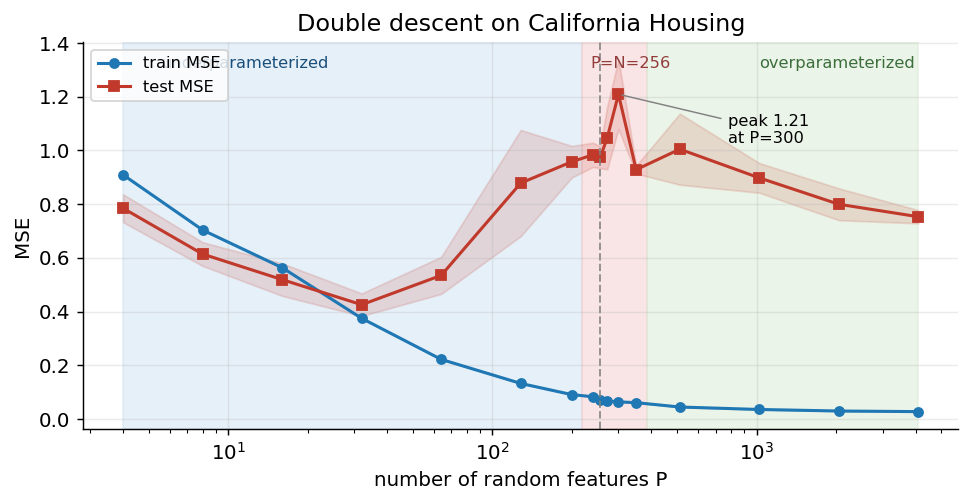
\includegraphics[width=0.82\linewidth]{regime_annotated.png}
\end{center}
\vspace{-3pt}
\footnotesize
$x$-axis is the number of random features $P$ on a log scale, $y$-axis is test MSE (lower is better). The shaded bands mark the underparameterized regime ($P \ll N$, blue), the interpolation threshold ($P \approx N$, red), and the overparameterized regime ($P \gg N$, green). The dashed line marks $P = N = 256$.
\begin{itemize}\setlength\itemsep{1pt}
\item Best in the underparameterized regime: $0.43$ at $P = 32$.
\item Spike at the interpolation threshold: $1.21$ at $P \approx 300$.
\item Second descent in the overparameterized regime: $0.75$ at $P = 4096$.
\end{itemize}
\end{frame}

\begin{frame}{Each Factor Alone Collapses the Spike}
\begin{center}
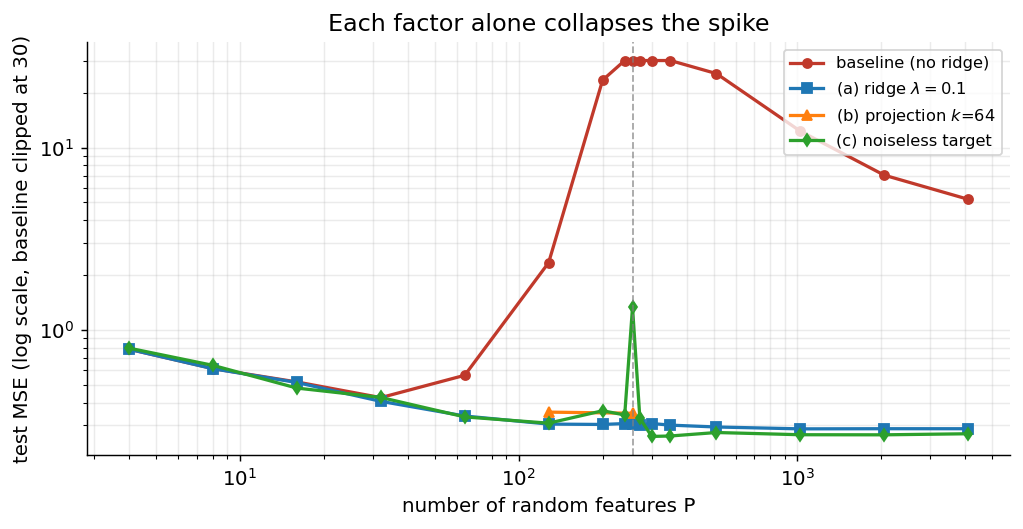
\includegraphics[width=0.82\linewidth]{factor_overlay.png}
\end{center}
\vspace{-3pt}
\footnotesize
All four conditions are plotted on the same log-$y$ axis (lower is better). The \textcolor{baseline}{\textbf{red baseline}} curve has the spike at $P = N$. The \textcolor{ridge}{\textbf{blue}}, \textcolor{proj}{\textbf{orange}}, and \textcolor{noise}{\textbf{green}} curves are each one of the three Schaeffer factors applied alone. Each factor flattens the spike independently.
\end{frame}

\begin{frame}{The Headline Numbers at $P = N$}
\begin{center}
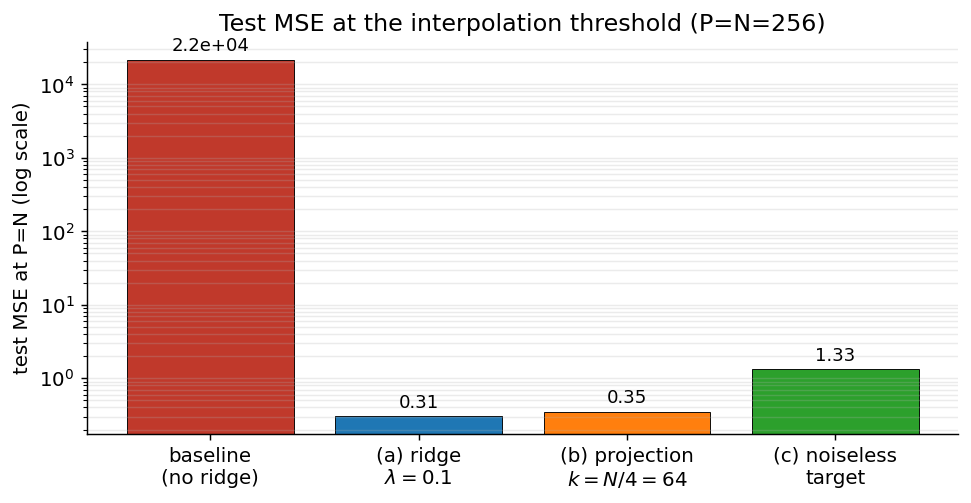
\includegraphics[width=0.72\linewidth]{factor_bars_at_N.png}
\end{center}
\vspace{-3pt}
\footnotesize
$y$-axis is test MSE at the interpolation threshold $P = N = 256$, on a log scale because the baseline is four orders of magnitude above the rest (lower is better).
\begin{itemize}\setlength\itemsep{0pt}
\item Baseline (no ridge) blows up to $\sim 2 \times 10^4$ from numerical instability ($\sigma_{\min} \to 0$).
\item Ridge $\lambda = 0.1$ collapses it to $0.31$. Four orders of magnitude.
\item Projection at $k = N/4$ matches it ($0.35$) without using $\lambda$.
\item Noiseless target alone reaches $1.33$. Less dramatic but still confirmatory.
\end{itemize}
\end{frame}

\begin{frame}{Spectral Collapse at $P = N$}
\begin{center}
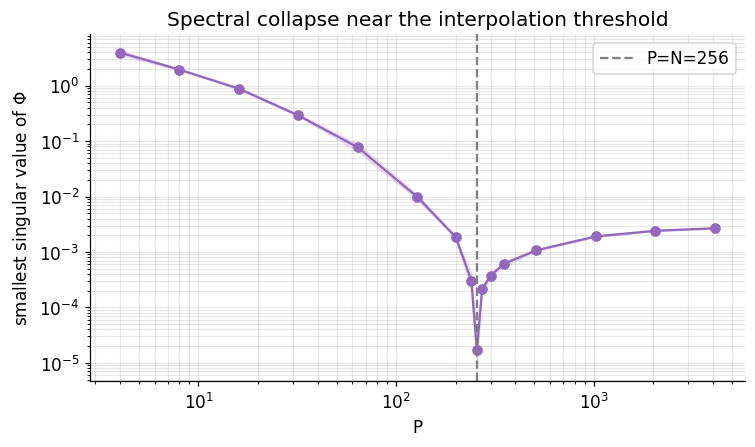
\includegraphics[width=0.65\linewidth]{smallest_singular_value.png}
\end{center}
\vspace{-3pt}
\footnotesize
Both axes are log-scale. $x$-axis is the number of random features $P$, $y$-axis is the smallest singular value $\sigma_{\min}$ of the random feature matrix $\Phi_{\text{train}}$. The matrix becomes invertible (and ridge regression well-conditioned) only when $\sigma_{\min}$ is comfortably above zero.
\begin{itemize}\setlength\itemsep{0pt}
\item $\sigma_{\min}$: $0.082$ at $P = 64$, drops to $6 \times 10^{-7}$ at $P = N$, recovers to $0.003$ at $P = 4096$.
\item The dip is exactly at the interpolation threshold.
\item Structural witness for factor (a). The small singular value is what ridge stabilizes.
\end{itemize}
\end{frame}

\begin{frame}{Random Features Approximate Exact RBF Kernel Ridge}
\begin{center}
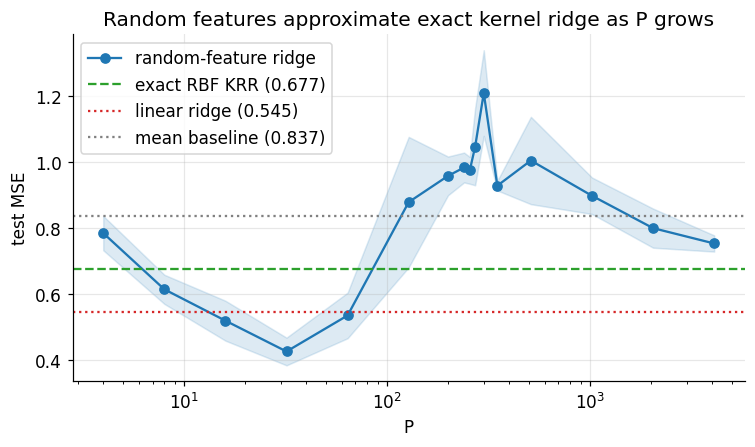
\includegraphics[width=0.6\linewidth]{kernel_approximation.png}
\end{center}
\vspace{-3pt}
\scriptsize
The blue curve is the random-feature ridge sweep across $P$ (lower is better). Horizontal lines are fixed-MSE values for the three reference baselines. The curve approaching a horizontal line means random features are approximating that method.
\begin{itemize}\setlength\itemsep{0pt}
\item Random-feature ridge approaches the exact RBF kernel ridge line as $P$ grows. The approximation works.
\item Linear ridge wins ($0.55$). California Housing has strong linear structure and RBF at the median bandwidth is not competitive.
\item Approximation point and kernel-choice point are separate. The first holds. The second doesn't.
\end{itemize}
\end{frame}

\begin{frame}{Singular Spectrum at Varying $P$}
\begin{center}
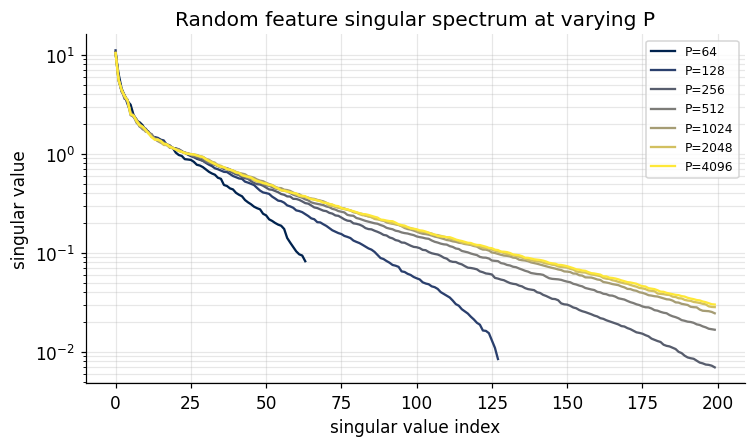
\includegraphics[width=0.65\linewidth]{kpca_spectrum.png}
\end{center}
\vspace{-3pt}
\footnotesize
\scriptsize
Each colored curve is the full singular spectrum of $\Phi_{\text{train}}$ at one fixed $P$. $x$-axis is the singular value index (largest first), $y$-axis is the singular value on a log scale. A curve crashing toward the bottom means many near-zero singular values, the geometric source of double descent.
\begin{itemize}\setlength\itemsep{0pt}
\item As $P$ grows the spectrum lengthens. Near $P = N$ the trailing tail collapses to numerical zero.
\item In the overparameterized regime the bulk is preserved and the tail recovers.
\end{itemize}
\end{frame}

% ============================================================
\section{Discussion}
% ============================================================

\begin{frame}{Putting the Story Together}
\footnotesize
\textbf{Going back to the central question.} Where does the classical bias-variance curve break?
\vfill
\textbf{Answer.} It breaks because the ridgeless interpolator at $P = N$ is built on top of a near-singular feature matrix. The spike is a consequence of that singularity, and any of three independent fixes can remove it.
\vfill
\begin{enumerate}\setlength\itemsep{1pt}
\item Test MSE peaks at $P \approx 300$ (just past $N = 256$) at $1.21$, then descends to $0.75$ at $P = 4096$.
\item \textcolor{ridge}{Ridge $\lambda = 0.1$} collapses the spike from $\sim 2 \times 10^4$ to $0.31$.
\item \textcolor{proj}{Projection at $k = N/4$} reaches $0.35$ without using $\lambda$.
\item \textcolor{noise}{Noiseless target} alone reaches $1.33$.
\item Smallest singular value of $\Phi_{\text{train}}$ collapses to $6 \times 10^{-7}$ exactly at $P = N$. This is the structural witness.
\end{enumerate}
\end{frame}

\begin{frame}{Limitations}
\footnotesize
\begin{itemize}\setlength\itemsep{3pt}
\item \textbf{Single dataset, single kernel.} California Housing with the RBF kernel only. The picture may differ on data with weaker linear structure or with kernels other than RBF.
\item \textbf{No bandwidth tuning.} $\sigma$ is set by the median heuristic only. A tuned bandwidth might close the gap to linear ridge.
\item \textbf{Three-factor ablations done one at a time.} Factorial combinations are needed to isolate each factor's contribution from the others.
\item \textbf{Small training subset ($N = 256$).} Chosen to make the interpolation threshold cheap to span, but classical bias-variance behavior may differ at $N$ in the thousands.
\end{itemize}
\end{frame}

\begin{frame}{Future Work}
\footnotesize
\begin{itemize}\setlength\itemsep{3pt}
\item \textbf{Synthetic data with controlled noise.} Lets factor (c) be tested cleanly with known signal-to-noise ratio.
\item \textbf{Tuned bandwidths and additional kernels.} Tests whether the linear-wins-on-California-Housing result is bandwidth-specific or kernel-specific.
\item \textbf{Larger $N$ grids.} Sweep $N$ to test whether the three-factor account holds across regimes, not just at $N = 256$.
\item \textbf{Factorial three-factor combinations.} Run all $2^3 = 8$ combinations of (a, b, c) on/off to estimate each factor's marginal contribution.
\end{itemize}
\end{frame}

\begin{frame}{Five Takeaways}
\footnotesize
\begin{enumerate}\setlength\itemsep{2pt}
\item Double descent is reproducible on tabular data with a small training subset. Test MSE peaks at $P \approx 300$ (just past $N$) at $1.21$.
\item \textcolor{ridge}{\textbf{Ridge regularization}} is the most powerful single fix. $\lambda = 0.1$ collapses the spike from $\sim 2 \times 10^4$ to $0.31$.
\item \textcolor{proj}{\textbf{Leading-mode projection}} at $k = N/4$ matches ridge ($0.35$) without using $\lambda$ at all.
\item The smallest singular value of $\Phi_{\text{train}}$ collapses to $6 \times 10^{-7}$ exactly at $P = N$. The dip is the structural source of the spike.
\item Random Fourier features genuinely approximate the RBF kernel as $P$ grows. Whether RBF is the right kernel for the data is a separate question.
\end{enumerate}
\end{frame}

\begin{frame}
\begin{center}
\Large\textbf{Questions?}

\vfill
\normalsize
Nicholas Welsh \\
\texttt{nwelsh2024@my.fit.edu} \\
\vspace{0.5cm}
\href{https://github.com/nickvpn/vit-ml-xai-project}{github.com/nickvpn/vit-ml-xai-project}
\end{center}
\end{frame}

\end{document}
